%% The comment character in TeX / LaTeX is the percent character.
%% The following chunk is called the header

\documentclass{article} % essential first line
\usepackage{times}    % this uses fonts which will look nice in PDF format
\usepackage{graphicx}   % needed for the figures
\usepackage{url}
\usepackage{adjustbox}
\usepackage{amsmath}
\usepackage{listings}
\usepackage{color}

\definecolor{dkgreen}{rgb}{0,0.6,0}
\definecolor{gray}{rgb}{0.5,0.5,0.5}
\definecolor{mauve}{rgb}{0.58,0,0.82}

\lstset{frame=tb,
  language=Java,
  aboveskip=3mm,
  belowskip=3mm,
  showstringspaces=false,
  columns=flexible,
  basicstyle={\small\ttfamily},
  numbers=none,
  numberstyle=\tiny\color{gray},
  keywordstyle=\color{blue},
  commentstyle=\color{dkgreen},
  stringstyle=\color{mauve},
  breaklines=true,
  breakatwhitespace=true,
  tabsize=3
}

%% Set the folder where pictures are located
\graphicspath{ {figures/} }

%% Here I adjust the margins

\oddsidemargin -0.25in    % Left margin is 1in + this value
\textwidth 6.75in   % Right margin is not set explicitly
\topmargin 0in      % Top margin is 1in + this value
\textheight 9in     % Bottom margin is not set explicitly
\columnsep 0.25in   % separation between columns

%% Define a macro for inserting postscript images
%% ==============================================
%% This is a macro which nominally takes 3 parameters, 
%% it would be used as follows to insert and encapsulated postscript
%% image at the location where it is used.
%%
%% \EPSFIG{epsfilename}{caption}{label}
%% - epsfilename is the name of the encapsulated postscript file to be
%%               inserted at this location
%% - caption is the text to be shown as the figure caption, it will be
%%           prepended by Figure X.  The number X can be referenced
%%           using the label parameter.
%% - label is a name given to the figure, it can be referenced using the
%%         \ref{label} command.

%\def\EPSFIG[#1]#2#3#4{   % Don't be scared by this monsrosity
%\begin{figure}[hbt]    % it is a macro to save typing later
%\begin{center}     % 
%\includegraphics[#1]{#2} %
%\end{center}     %
%\caption{#3}     %
%\label{#4}     %
%\end{figure}     %
%}        %

%% Define the fields to be displayed by a \maketitle command
\author{Timothy Dee, Brent Barth}
%{\it Undergraduate, Department of Electrical and Computer Engineering, Iowa State University}
%\author{Brent Barth}
%\it Undergraduate, Department of Electrical and Computer Engineering, Iowa State University}
\title{Lab 1 Report}

%%
%% Header now finished
%%

\begin{document}    % Critical
\twocolumn
\thispagestyle{empty}   % Inhibit the page number on this page
\maketitle      % Use the \author, \title and \date info

%% Next comes the abstract, notice the curly-braces surrounding the
%% text.

\abstract{This report contains a description and analysis of the findings during Lab 1 of CprE 458, Real Time Systems. Contained herein is all relevant program code, and the results from having run this code. Results measure the effect of varying processor frequency control mechanisms on energy consumption and computation time.}

\section{Introduction}
This paper has sections discussing theory, program code, energy consumption data analysis, and analysis of computation time. Each of these sections discuss design decisions and the motivation behind those decisions those decisions were made.
The interesting component to this lab is that it has some clear real world applications. We are able to see how the processor frequency has an effect on both performance and energy consumption. 
This gives insight into design decisions which are made about processors in mobile devices. For example, the processors in mobile devices tend to be designed to run at a lower frequency than a desktop computer. This makes sense as power consumption increases with frequency. 

% theory of:
% how processor frequency affects power consumption
% how processor frequency affects computation time
% lecture 10 contains the relevant information
\section{Theory}
We have learned about varying strategies for decreasing power consumption in mobile systems. 
The power consumption of a processor depends both on the voltage applied to the processor, and the frequency at which the processor is run. Following from this fact are two unique strategies of minimizing the power consumed by a processor. One strategy requires varying the voltage applied to the processor. This method is used by the Apple A7 and Qualcomm Snapdragon processors. 
Another method is reducing the frequency of the processor when execution at a higher frequency provides small or no benefit. Situations where the device is underloaded are good candidates for reducing the frequency.

\subsection{Power Consumption}
Power consumed by a processor is related to frequency of the processor by $P \propto V^2*F$ where $P$ is power consumed, $V$ is voltage, and $F$ is frequency at which the processor is ran.
This relationship implies power consumption increases as frequency and voltage increase. From this we deduce that decreasing the frequency or voltage will yield a net decrease in the power consumption. 

Decreasing the frequency has an effect on the runtime of tasks. A lower frequency means tasks will run slower. Thus we are wise to consider the total energy consumed by a task instead of just its $P = \frac{energy}{time}$.
Consider a task $T$ run at two different frequencies, $F_{1}$ and $F_{2}$. Where $F_{2} = F_{1}*2.$.
Energy consumed by task is $E_{T} = K*CC*F^2$ where $CC$ is the number of clock cycles task $T$ will take and $K$ is a constant. In this case the ratio of energy taken to compute the task at frequency $F_{2}$ compared to frequency $F_{1}$ is $\frac{K*CC*F_{2}^2}{K*CC*F_{1}^2} = \frac{K*CC*4*F_{1}^2}{K*CC*F_{1}^2} = 4$.

In this particular situation it takes four times as much energy to execute this task at the higher frequency. This result shows an exponential increase in the energy usage with increases in frequency. This exponential increase represents the general relationship between energy consumption and processor frequency.

\subsection{Computation Time}
In this lab exercise we explore how computation time is affected by the adjustment of the processor frequency.
Computation time of a task $T$ can be represented by $\frac{CC}{F}$ where CC is the number of clock cycles in task $T$ and $F$ is the frequency at which the task is run.
This relationship implies there should be a linear decrease in the computation time as frequency increases.

\section{Part 1 - Code}
\subsection{High Performance Mode}
\begin{lstlisting}[float=*, caption={High Performance Mode},label={lst:HPM},numbers=left]
PMbutton2.setOnClickListener(new View.OnClickListener() {

      @Override
      public void onClick(View v) {

        OPERATIONmessage("[High Performance Mode] ###########################################");
        //TODO Please program for High Performance Mode here (done)

        DATAname = "1300000"; // Setting up the minimum frequency 1300 Mhz
        DATAaddress = "/sys/devices/system/cpu/cpu0/cpufreq/scaling_min_freq";
        ChangeCPUinfor(CPUname, DATAname, DATAaddress);
        DATAname = "1300000"; // Setting up the maximum frequency at 1300 MHz
        DATAaddress = "/sys/devices/system/cpu/cpu0/cpufreq/scaling_max_freq";
        ChangeCPUinfor(CPUname, DATAname, DATAaddress);

        CPUname = "High Power";
        DATAname = "current min frequency";
        DATAaddress = "/sys/devices/system/cpu/cpu0/cpufreq/scaling_min_freq";
        ReadCPUinfor(CPUname, DATAname, DATAaddress);
        DATAname = "current MAX frequency";
        DATAaddress = "/sys/devices/system/cpu/cpu0/cpufreq/scaling_max_freq";
        ReadCPUinfor(CPUname, DATAname, DATAaddress);

        OPERATIONmessage("[High Performance Mode] ###########################################");


      }
    });
\end{lstlisting}
Listing \ref{lst:HPM} describes our implementation of high performance mode. This code was straightforward due to its similarity with low performance mode.

\subsection{Dynamic Frequency Scaling}
\begin{lstlisting}[caption={Dynamic Frequency Scaling Mode Execution},label={lst:DFS_thread},numbers=left]
button_pressed=true;

        (new Thread() {
          public void run() {
            // do stuff

        while(button_pressed == true) {
          // mode values table
          // value : meaning
          // 1 : Dynamic Frequency Scaling Mode I
          // 2 : Dynamic Frequency Scaling Mode II
          // 3 : Dynamic Frequency Scaling Mode Mixed
          int mode = 3;

          // determine the current load of the processors
          double load = ReadCPUload();

          //call functions which implement the different Dynamic Frequency scaling Modes
          if (mode == 1) {
            setDFS_1(load);
          } else if (mode == 2) {
            setDFS_2();
          } else if (mode == 3) {
            setDFS_Mixed(load);
          }

          try {
            this.sleep(1000);
          }catch(Exception e){
            e.printStackTrace();
          }
        }
          }
        }).start();
\end{lstlisting}
An interesting problem in this lab exercise is getting the dynamic frequency scaling decisions to be made continuously. We had some difficulty doing this at first. Before we realized the need to set the values of the processor on a time interval, we were confused by why the processor value would always stay the same after the first call to Dynamic Frequency Scaling mode X.
Upon discovery of this design necessity we employed the following scheme. The code shown in Listing \ref{lst:DFS_thread} was employed to run the code for the DFS mode continuously until another frequency mode is selected. 
This is accomplished by using a while loop to run the DFS code on a new thread separate from the main thread. The condition of the while loop is a boolean variable. This boolean variable is set to true before the loop begins. When either of High Performance Mode button or Low Performance Mode buttons are pressed, this boolean variable is set to false.

\subsubsection{Dynamic Frequency Scaling Mode I}
\begin{lstlisting}[float=*,caption={Dynamic Frequency Scaling Mode I},label={lst:DFS_1},numbers=left]
private void setDFS_1(double cpu_load){
    // determine if I should go to a power mode
    if(cpu_load < .2){
      // go to low performance mode
      PMbutton1.performClick();
    }else if(cpu_load > .9){
      //go to high performance mode
      PMbutton2.performClick();
    }else{
      // set the frequency range between 51 Mhz and 1.3 Ghz
      DATAname = "51000"; // Setting up the minimum frequency 51 Mhz
      DATAaddress = "/sys/devices/system/cpu/cpu0/cpufreq/scaling_min_freq";
      ChangeCPUinfor(CPUname, DATAname, DATAaddress);
      DATAname = "1300000"; // Setting up the maximum frequency at 1300 MHz
      DATAaddress = "/sys/devices/system/cpu/cpu0/cpufreq/scaling_max_freq";
      ChangeCPUinfor(CPUname, DATAname, DATAaddress);

      CPUname = "Dynamic Mode";
      DATAname = "current min frequency";
      DATAaddress = "/sys/devices/system/cpu/cpu0/cpufreq/scaling_min_freq";
      ReadCPUinfor(CPUname, DATAname, DATAaddress);
      DATAname = "current MAX frequency";
      DATAaddress = "/sys/devices/system/cpu/cpu0/cpufreq/scaling_max_freq";
      ReadCPUinfor(CPUname, DATAname, DATAaddress);
    }
  }
\end{lstlisting}
Listing \ref{lst:DFS_1} describes our implementation of dynamic frequency scaling mode I. This mode varies the frequency range according to according to the CPU load. Lower processor frequencies will conserve power while higher processor frequencies will allow for increased performance. 
Certain CPU loads require that the processor be set to high performance mode or low performance mode. To accomplish this we use the performClick() method attached to the low performance mode and high performance mode buttons. This has the same effect as the user pressing the button which corresponds to these modes.

\subsubsection{Dynamic Frequency Scaling Mode II}
\begin{lstlisting}[float=*,caption={Dynamic Frequency Scaling Mode II},label={lst:DFS_2},numbers=left]
  private void setDFS_2(){
    // get the battery level
    IntentFilter ifilter = new IntentFilter(Intent.ACTION_BATTERY_CHANGED);
    Intent batteryStatus = this.registerReceiver(null, ifilter);

    int level = batteryStatus.getIntExtra(BatteryManager.EXTRA_LEVEL, -1);
    int scale = batteryStatus.getIntExtra(BatteryManager.EXTRA_SCALE, -1);

    float battery_percent = level / (float)scale;

    // determine whether the screen is on
    boolean is_display_on = false;
    DisplayManager dm = (DisplayManager) this.getSystemService(Context.DISPLAY_SERVICE);
    for (Display display : dm.getDisplays()) {
      if (display.getState() != Display.STATE_OFF) {
        is_display_on = true;
      }
    }

    // get the charging state
    int status = batteryStatus.getIntExtra(BatteryManager.EXTRA_STATUS, -1);
    boolean is_charging = status == BatteryManager.BATTERY_STATUS_CHARGING ||
        status == BatteryManager.BATTERY_STATUS_FULL;

    //(continued on next page)    
\end{lstlisting}
\begin{lstlisting}[float=*,caption={Dynamic Frequency Scaling Mode II (continued)},label={lst:DFS_2_2},numbers=left]
// determine if we are charging
    if(is_charging){
      // if we are charging we don't care about power usage.... set to high performance mode
      setHighPerformanceMode();
      Log.d("high","performance");
    }else if(battery_percent < .3) {
      // we want to conserve energy because we are almost out of it, set to low performance mode
      setLowPerformanceMode();
      Log.d("low","performance");
    }else{
        // if we're not charging and not low battery we have some decisions to make
        // if the wireless radio is on we are likely doing something online.
        // If we are doing something we will like a more responsive device
        // so allow the processor to vary between two fairly high frequency states
        if (is_display_on) {
          // set to fairly high processing state
          // set the frequency range between 700 Mhz and 1.3 Ghz
          DATAname = "700000"; // Setting up the minimum frequency 51 Mhz
          DATAaddress = "/sys/devices/system/cpu/cpu0/cpufreq/scaling_min_freq";
          ChangeCPUinfor(CPUname, DATAname, DATAaddress);
          DATAname = "1300000"; // Setting up the maximum frequency at 1300 MHz
          DATAaddress = "/sys/devices/system/cpu/cpu0/cpufreq/scaling_max_freq";
          ChangeCPUinfor(CPUname, DATAname, DATAaddress);

          CPUname = "Dynamic Mode";
          DATAname = "current min frequency";
          DATAaddress = "/sys/devices/system/cpu/cpu0/cpufreq/scaling_min_freq";
          ReadCPUinfor(CPUname, DATAname, DATAaddress);
          DATAname = "current MAX frequency";
          DATAaddress = "/sys/devices/system/cpu/cpu0/cpufreq/scaling_max_freq";
          ReadCPUinfor(CPUname, DATAname, DATAaddress);
        } else {
          // set to lower processing state
          // set the frequency range between 51 Mhz and 700 Mhz
          DATAname = "51000"; // Setting up the minimum frequency 51 Mhz
          DATAaddress = "/sys/devices/system/cpu/cpu0/cpufreq/scaling_min_freq";
          ChangeCPUinfor(CPUname, DATAname, DATAaddress);
          DATAname = "700000"; // Setting up the maximum frequency at 1300 MHz
          DATAaddress = "/sys/devices/system/cpu/cpu0/cpufreq/scaling_max_freq";
          ChangeCPUinfor(CPUname, DATAname, DATAaddress);

          CPUname = "Dynamic Mode";
          DATAname = "current min frequency";
          DATAaddress = "/sys/devices/system/cpu/cpu0/cpufreq/scaling_min_freq";
          ReadCPUinfor(CPUname, DATAname, DATAaddress);
          DATAname = "current MAX frequency";
          DATAaddress = "/sys/devices/system/cpu/cpu0/cpufreq/scaling_max_freq";
          ReadCPUinfor(CPUname, DATAname, DATAaddress);
        }
      Log.d("Moderate","Performance");
    }
  }
\end{lstlisting}
Listings \ref{lst:DFS_2} and \ref{lst:DFS_2_2} show our implementation of dynamic frequency scaling mode 2. For this mode we though about the phone states which affect the scarcity of power. We determined that the screen state (on or off) and the charging state of the phone were significant enough to be determining factors in how we choose to manage the processor frequency.

In the case of the screen state the following train of logic was applied. If the screen is on, then we are likely to be interacting with an application. If we are interacting with an application than we will certainly benefit from a more responsive device. Therefore we elect to put the phone in a higher power state while the screen is on. We save energy by setting the phone in a lower power state when the screen radio is off.
The decision making for the charging state is straightforward. If the phone is charging then we don't need to worry about power consumption, even if the battery is low.

\subsubsection{Dynamic Frequency Scaling Mode Mixed}
\begin{lstlisting}[float=*,caption={Dynamic Frequency Scaling Mode Mixed},label={lst:DFS_mixed},numbers=left]
  private void setDFS_Mixed(double cpu_load) {
    // get the battery level
    IntentFilter ifilter = new IntentFilter(Intent.ACTION_BATTERY_CHANGED);
    Intent batteryStatus = this.registerReceiver(null, ifilter);

    int level = batteryStatus.getIntExtra(BatteryManager.EXTRA_LEVEL, -1);
    int scale = batteryStatus.getIntExtra(BatteryManager.EXTRA_SCALE, -1);

    float battery_percent = level / (float)scale;

    // get the charging state
    int status = batteryStatus.getIntExtra(BatteryManager.EXTRA_STATUS, -1);
    boolean is_charging = status == BatteryManager.BATTERY_STATUS_CHARGING ||
        status == BatteryManager.BATTERY_STATUS_FULL;

    // determine if we are charging
    if(is_charging){
      // if we are charging we don't care about power usage.... set to high performance mode
      setHighPerformanceMode();
    }else {
      // vary the processor frequency based on the battery level.
      // the higher the battery level, the higher the frequency.
      // anywhere from 100000 khz to 1300000 khz
      double step_size = 1.0/12.0;

      // pretend like the cpu_load is less if the battery percent is lower
      int load_fraction = new Double(Math.ceil( (cpu_load * battery_percent) / step_size)).intValue();

      // load_fraction is at greatest 1
      int high_frequency = 100000 * (Integer.valueOf(load_fraction) + 1);
      int low_frequency = high_frequency;

      Log.d("low_frequency",new Integer(low_frequency).toString());
      Log.d("high_frequency", new Integer(high_frequency).toString());

      // set to fairly high processing state
      DATAname = String.valueOf(low_frequency); // Setting up the minimum frequency at low frequency
      DATAaddress = "/sys/devices/system/cpu/cpu0/cpufreq/scaling_min_freq";
      ChangeCPUinfor(CPUname, DATAname, DATAaddress);
      DATAname = String.valueOf(high_frequency); // Setting up the maximum frequency at high frequency
      DATAaddress = "/sys/devices/system/cpu/cpu0/cpufreq/scaling_max_freq";
      ChangeCPUinfor(CPUname, DATAname, DATAaddress);

      CPUname = "Dynamic Mode";
      DATAname = "current min frequency";
      DATAaddress = "/sys/devices/system/cpu/cpu0/cpufreq/scaling_min_freq";
      ReadCPUinfor(CPUname, DATAname, DATAaddress);
      DATAname = "current MAX frequency";
      DATAaddress = "/sys/devices/system/cpu/cpu0/cpufreq/scaling_max_freq";
      ReadCPUinfor(CPUname, DATAname, DATAaddress);
    }
  }
\end{lstlisting}
Listing \ref{lst:DFS_mixed} shows our implementation of dynamic frequency scaling mode mixed. For this mode we choose to use the charging state, battery charge percent, and cpu load as determining factors in our algorithm. All of these factors have a significant impact on how much we care about our energy usage. In many cases we are willing to sacrifice energy in exchange for performance.

As discussed previously, the charging state impacts our decisions in a straightforward way. If the device is being charged than we do not have to worry about power consumption, and we can activate high performance mode. When the device is not charging set a frequency range as a function of charge percent and cpu load.
We set load fraction to be an integer ranging between 0 and 12 depending on the cpu load. A load fracting of 0.0 yields 100000 Khz processor frequency while a load fraction of 12 yields 1300000 Khz processor frequency. load fraction increases linearly with cpu load and decreases linearly with battery percent.
battery percent causes the program to pretend like the cpu load is smaller than reality.

\subsection{Measuring Computation Time}
\begin{lstlisting}[caption={Measuring Computation Time - Intense Task Launcher},label={lst:MCT_launcher},numbers=left]
  private long result_factorial;
  private void intense_computation(){
    int computation = 3;

    // do factorial of n recursivly, measure computation time
    long before_time = SystemClock.currentThreadTimeMillis();

    result_factorial=11111l;
    long n = 33;
    for(int i=0;i<50;i++) {
      if(computation == 1) {
        recursive_factorial(n);
      }else if(computation == 2){
        square_big_numbers(n);
      }else {
        fibonacci(n);
      }
    }

    long run_time = SystemClock.currentThreadTimeMillis() - before_time;

    Log.d("Factorial Result", new Long(result_factorial).toString());

    //print the run_time as op message
    OPERATIONmessage2("Run Time" + run_time);
  }
\end{lstlisting}
Listing \ref{lst:MCT_launcher} depicts the code we used to measure computation time under each of the different modes. Depending on the value of the computation variable, the code will run one of three computationally intense functions. These functions constitute each of the loads we tested for computation time. When running the code we had to vary the number of times the for loop ran in order to make the computation time manageable. 
We ran recursive\_factorial() ten million times, square\_big\_numbers() ten million times, and fibonacci() 50 times. Each of these tests took about ten seconds to run.

\begin{lstlisting}[caption={Measuring Computation Time - Sum of Squares},label={lst:MCT_square_sum},numbers=left]
  private long square_big_numbers(long n){
    if(n <= 1 ){
      return 1;
    }

    return square_big_numbers(n-1) + n^2;
  }
\end{lstlisting}
Listing \ref{lst:MCT_square_sum} depicts a test which computes the sum on the square of all the numbers from 1 to n. This constitutes a significant computation when it is run ten million times.

\begin{lstlisting}[caption={Measuring Computation Time - Fibonacci},label={lst:MCT_fibonacci},numbers=left]
private long fibonacci(long number){
    if ((number == 0) || (number == 1)) // base cases
      return number;
    else
      return fibonacci(number - 1) + fibonacci(number - 2);
  }
\end{lstlisting}
Listing \ref{lst:MCT_fibonacci} depicts a test which computes the nth fibonacci number. This constitutes a significant computation when it is run fifty times.

\begin{lstlisting}[caption={Measuring Computation Time - Factorial},label={lst:MCT_factorial},numbers=left]
  private long recursive_factorial(long i){
    if(i <= 1){
      return 1;
    }

    return recursive_factorial(i-1)*i;
  }
\end{lstlisting}
Listing \ref{lst:MCT_factorial} depicts a test which computes the factorial of n. This constitutes a significant computation when it is run ten million times.

\subsection{Computing CPU Load}
\begin{lstlisting}[caption={Computing CPU Load},label={lst:cpu_load},numbers=left]
protected double ReadCPUload() {

    ProcessBuilder cmd;
    double result=0.0;

    try{

      String[] args = {"/system/bin/cat", "/proc/stat"};
      cmd = new ProcessBuilder(args);

      Process process = cmd.start();
      InputStream in = process.getInputStream();
      byte[] re = new byte[1024];
      String stat = "";

      while(in.read(re) != -1) {
        stat += new String(re);
        //read the entire input strea
        //result = result + new String(re);
      }

      in.close();

      // parse stat for the load data
      String load;
      Scanner stat_scanner = new Scanner(stat);

      load = stat_scanner.nextLine();
      String[] toks = stat_scanner.nextLine().split(" ");

      //do the cpu load calculation based on the first line of /proc/stat
      int user_time = Integer.valueOf(toks[1]);
      int nice_time = Integer.valueOf(toks[2]);
      int system_time = Integer.valueOf(toks[3]);
      int idle_time = Integer.valueOf(toks[4]);
      int iowait = Integer.valueOf(toks[5]);
      int irq = Integer.valueOf(toks[6]);
      int softirq = Integer.valueOf(toks[7]);
      int steal = Integer.valueOf(toks[8]);
      int guest = Integer.valueOf(toks[9]);
      int guest_nice = Integer.valueOf(toks[10]);

      // Guest time is already accounted in usertime
      int usertime = user_time - guest;
      int nicetime = nice_time - guest_nice;
      // Fields existing on kernels >= 2.6
      // (and RHEL's patched kernel 2.4...)
      int idlealltime = idle_time + iowait;
      int systemalltime = system_time + irq + softirq;
      int virtalltime = guest + guest_nice;
      int totaltime = usertime + nicetime + systemalltime + idlealltime + steal + virtalltime;

      result = ((double)(totaltime - idlealltime))/totaltime;
      OPERATIONmessage2("CPU load = "+ result + "\n");
    } catch(IOException ex){
      ex.printStackTrace();
    } catch(Exception e){
      e.printStackTrace();
    }
    Log.d("cpu_load", Double.toString(result));
    return result;
  }
\end{lstlisting}
Listing \ref{lst:cpu_load} shows the process for computing cpu load from the information given in the /proc/stat file. The information in this file is used to compute the percentage of the CPU which is currently utilized by tasks.

%we should say how we did each of the tests. We should also say what we used to generate each of the loads.
\section{Part 2 - Data Analysis}
%possibly insert a table indicating what energy consumption we got for each energy scheme under each load.
%might also be useful to include description of the testing.
%must include graphs of each test result
\subsection{Measuring energy consumption}
The PowerTutor application suggested in the laboratory description is used to gather the data presented in this section. Three different loads were applied to the Nexus 7 tablet while it was set to each of the power modes. We observe both the time a task takes to run and the average power consumption during the time period the application ran. Together these figures allow us to compute the total energy consumed by the task as $E_{total} = P_{average}*T$ where $E$ is total energy, $P$ is average power consumed by the task, and $T$ is the time taken by the task.

\subsection{Comparison and Analysis}
\begin{figure}[!hbt]
\begin{center}
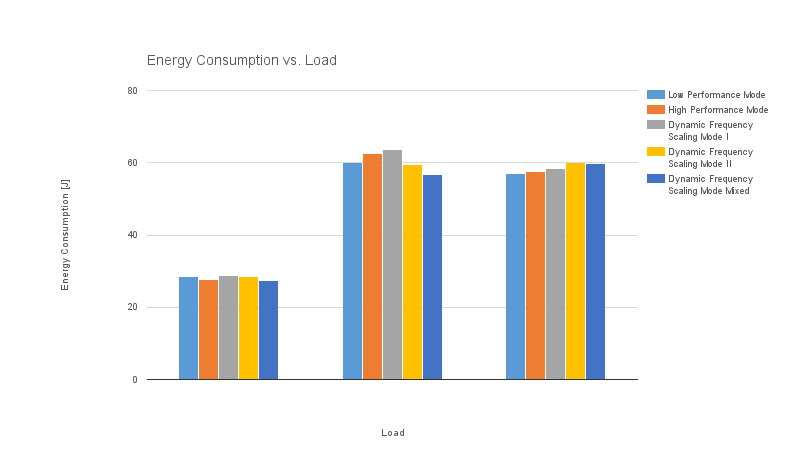
\includegraphics[width=.4\textwidth,keepaspectratio]{energy_vs_load.png}
\end{center}
\caption{fig:Energy Vs Load}
\label{FIG-TRANSMITTER}
\end{figure}

There are three different loads we used with our five different modes.  Load \#1 was a 30 second Youtube video, load \#2 was 30 seconds playing Temple Run game on the Nexus, and load \#3 was recording a video.  According to our results, we found difficulty determining much difference in the results from Load \#1.  Looking at our graph the low performance had higher energy consumption than high power which isn’t what is expected.  The Scaling modes performed as expected in Load \#1.  For Load \#2, the low and high performance performed as expected.  The high performance mode used more energy than the low energy mode.  The scaling modes performed as expected in this simulation.  The dynamic scaling mixed mode is being the most efficient in both loads by using the least amount of energy.  Load \#3 did worked as expected for the low and high power modes.  The high power consumed more energy because it used the higher frequency than the lower energy mode.  As for the scaling modes, 1 and 2 are working correctly, but the mixed mode used the most energy so it did not work as intended.  Even though each of these measured loads were consistent in the way we measured them, we cannot account for the other processes in the CPU and what the Android operating system is doing in the background.  Therefore we feel some error could be gaged towards this.  

\section{Extra Part - Measuring Computation Time}
\begin{figure}[!hbt]
\begin{center}
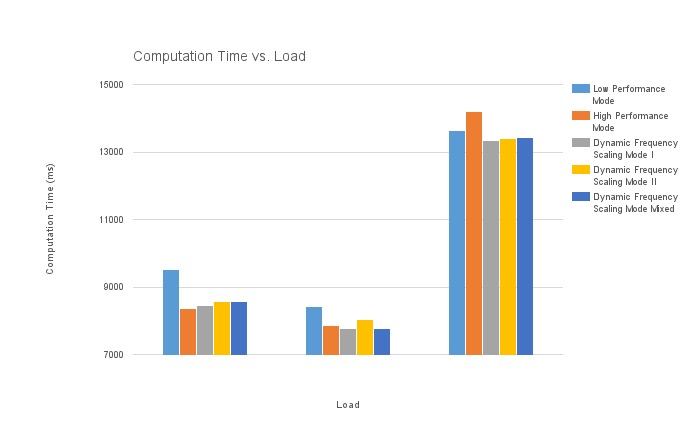
\includegraphics[width=.4\textwidth,keepaspectratio]{time_vs_load.png}
\end{center}
\caption{fig:Computation Time Vs Load}
\label{FIG-TRANSMITTER}
\end{figure}
We created three different loads to use with our five different power modes.  Load \#1 is computing 33!, 10000000 times, the load \#2 is sum the squares of the numbers up to 33, 10000000 times, and load \#3 is computing the 3rd Fibonacci number 50 times.  For Load \#1 the expected results were not comparable with the results we achieved.  The low performance mode used more time than the high performance.  The scaling modes were all similar to the expected results.  For Load \#2 the low and high performance ran as expected due to the higher frequency in the CPU for the high performance.  The Scaling modes all stayed similarly close.  The scaled mix mode also took the least amount of time to run which is expected.  The last load did not run as expected for the low and high performance.  The low performance ran faster than the high performance.  The scaling modes all about ran the same.  Other than the third load, the majority of our results line up with the theoretical results.  

% we should sum up the results
\section{Conclusion}
From this lab we learned how frequency can affects the CPU power consumption and time of the computations.  By using these different modes we were able to get real data about how frequency influences CPU time.  The low and high power frequency modes allow us to see the change that the higher frequencies have over the lower frequencies on the CPU.  The higher frequency has a lower computation time, but uses more power.  The lower frequency mode takes longer for computation time while it uses less power.  We also were able to see how different events such as low battery, radio state, charging, and CPU load can be used to differentiate the frequency provided for the CPU.  The scaling modes tended to run about the same for computation time and energy consumption.  This could be due to similar frequencies in the setup of the scale modes.  After looking at our results we feel that the scaling mixed mode would be the most beneficial.  This is because it based on the CPU load at that moment and the results from our labs show that.  This lab used the theory of CPU load we learned from class, and incorporated real life situations that we can measure on the mobile devices.  

%% This bit generates the references.  This part starts to get
%% slightly tricky.
\bibliographystyle{unsrt} % Order by citation
\bibliography{report}

\end{document}